
\begin{figure}
    \centering
    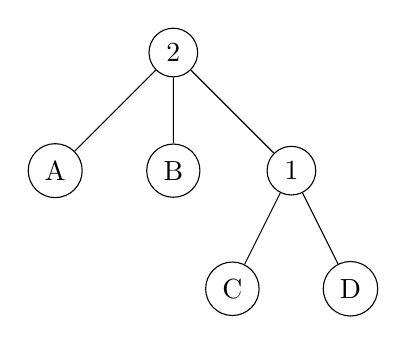
\begin{tikzpicture}
        \scoped{
                \tikzstyle{every node}=[circle, draw];
                \draw (0,0) node (root) [anchor=south] {2} child {node (a) {A}} child {node (b) {B}} child  {node (subroot) {1} child  {node (c) {C}} child  {node (d) {D}}};
            };
    \end{tikzpicture}
    \caption[Sample Access Tree]{
        Sample Access Tree over the attributes \texttt{A}, \texttt{B}, \texttt{C}, \texttt{D}.
    }
    \label{fig:sample-access-tree}
\end{figure}